\documentclass[journal]{IEEEtran}
\IEEEoverridecommandlockouts
\usepackage{cite}
\usepackage{amsmath,amssymb,amsfonts}
\usepackage{algorithmic}
\usepackage{graphicx}
\usepackage{textcomp}
\usepackage{xcolor}
\usepackage{booktabs}
\usepackage{multirow}
\usepackage{balance}
\usepackage[hidelinks]{hyperref}

\def\BibTeX{{\rm B\kern-.05em{\sc i\kern-.025em b}\kern-.08em
    T\kern-.1667em\lower.7ex\hbox{E}\kern-.125emX}}

\begin{document}

\title{Multilingual Spam Email Detection for English and Bangla Messages Using QLoRA-Fine-Tuned Large Language Models with Explainable AI Validation}

\author{Najmush~Shakib
        and~Munim~Halder% <-this % stops a space
\thanks{N. Shakib and M. Halder are with the Department of Computer Science and Engineering, Bangladesh University of Business and Technology (BUBT), Dhaka, Bangladesh (e-mail: nstasin81@gmail.com, munimhalder666@gmail.com).}%
}

\maketitle

\begin{abstract}
\normalfont
The advent of global messaging platforms has come together with a surge in spam, phishing, and smishing, which create a substantial burden in terms of financial and security costs for individuals around the globe. While spam detection algorithms have improved substantially for high-resource languages such as English, there is still an ongoing issue with low-resource languages like Bangla, spoken by more than 230 million people and poorly supported by existing commercial and academic spam filter products. Here we introduce a combined multilingual model for spam detection that is capable of classifying English and Bangla texts simultaneously without requiring feature engineering per language or having two separate pipelines. This work uses Quantized Low-Rank Adaptation (QLoRA) technique to adapt five small pretrained Large Language Models---Phi-3.5 Mini, Qwen2.5-1.5B, TinyLlama-1.1B, StableLM-2-1.6B, and SmolLM2-360M---to a dataset containing spam examples from SMS Spam Collection and native Bangla phishing dataset. Extensive pre-processing includes Unicode normalizing, replacing URL tokens with placeholder and leakage-free, group-aware splits using GroupShuffleSplit based on templates. Synthetic Minority Over-sampling Technique (SMOTE) is used to address class imbalance only in the training set. Model evaluation is done in terms of overall and language-wise performance metrics---accuracy, precision, recall, F1-score, and the difference between two models is compared using McNemar statistical significance test. For validation that prediction made by model is based on semantically relevant tokens, an Explainable AI (XAI) module that uses cross-layer attention aggregation technique is implemented. It is demonstrated that QLoRA fine-tuning of small LLMs is an extremely efficient way to build a spam detection model in terms of parameters. Moreover, the presented methodology is state-of-the-art for bilingual spam detection task, far outperforming machine learning algorithms reported in previous works.
\end{abstract}

\begin{IEEEkeywords}
Spam Detection, Bangla NLP, QLoRA, Large Language Models, Parameter-Efficient Fine-Tuning, PEFT, Explainable AI, Multilingual Classification, Phishing Detection, Smishing
\end{IEEEkeywords}

\section{Introduction}

\subsection{Background and Motivation}

Unwanted electronic messages, known collectively as spam, constitute a
significant and economically impactful security challenge in today's
digital communication environment. Spam messages do more than cause
irritation; they are used to launch phishing attacks, propagate malware,
send fraudulent financial offers, and conduct other malicious activities
from which billions of dollars worth of annual losses are incurred~\cite{ref1}. The increasing prevalence of mobile messaging applications such
as SMS, WhatsApp, and similar services has significantly expanded the
threat surface space, rendering ineffective previous approaches of rule
and keyword-based spam filtering techniques due to the use of
adversarial tactics such as linguistic variations and code switching~\cite{ref5},~\cite{ref6}.

Natural language processing (NLP) and machine learning (ML) have seen an incredible growth in their research domain and have generated many classifiers, which use statistical features, distributed word representations, recurrent neural networks, and lately transformer based pre-trained language models~\cite{ref4},~\cite{ref7},~\cite{ref9}. This progress has led detection accuracies for English language benchmarks to saturation levels with many current systems having accuracies above 98\% on well-established data sets such as SMS Spam Collection~\cite{ref1} and Enron Email~\cite{ref9}. However, the problem of generalization across languages is still a very serious issue and largely unaddressed challenge.

This challenge becomes especially pronounced in the example of the Bangla language, which is the seventh most spoken language in the world and the national language of Bangladesh. The digital communication medium in the country presents a combination of native Bangla script, romanized phonetic representation, English loan words and hybrid code switched construction. In addition, the presence of many mobile financial services (MFS) in the country like bKash and Nagad have resulted in development of localized context-based phishing attacks, which utilize knowledge about these platforms to lure victims. Current Bangla text classifiers, even those performing at high level on well-structured benchmark sets~\cite{ref7}, are often not designed to counter the emerging threat environment.

\subsection{Problem Statement}

Previous works usually divide into two kinds: resource-rich English
systems which are advanced but also linguistically exclusive, and
specialized Bangla systems which are innovative but exist in isolation
of other languages in the ever-evolving space of threat detection and
mitigation. The Bangla systems usually make use of deep learning models
which require huge amounts of annotated data, large amounts of
computational power, or specialized feature extraction that cannot
generalize to new attacks~\cite{ref7},~\cite{ref10}. No previous published system
handles English and Bangla spam in an integrated way using a unified
end-to-end model that does not employ language-specific pre-processing
streams or special tokenizers for Bangla.

However, this limitation is not merely academic in nature. In practical
applications where such a system could be used---a telecom company or
bank in a bilingual environment, for example---it is important to keep
in mind the extra cost and overhead of using multiple pipelines for each
language separately. Hence, the need for a unified model to handle raw
text in both languages and produce explainable classifications is
crucial.

\subsection{Proposed Solution and Contributions}

This work bridges this gap via introducing a single framework for
multilingual spam detection based on the fine-tuning of publicly
available compact Large Language Models (LLMs) via Quantized Low-Rank
Adaptation (QLoRA) \cite{ref11}. The QLoRA technique makes it possible to adapt
models with billions of parameters to specific classification problems
and only keep a small fraction of the initial parameters -- namely,
update less than 1\% of all the weights during training, thereby making
LLM fine-tuning possible on a single consumer GPU or even cloud-based
Jupyter notebook setup. This is especially important in the case of
low-resource languages, where computational limitations make fine-tuning
or even pre-training impossible.

Contributions of this paper include the following:

\textbf{(1) Unified Bilingual Classification Framework:} We design and test
the unified fine-tuned LLM-based pipeline for the joint problem of
English and Bangla spam detection that does not involve any
language-specific branching or feature extraction.

\textbf{2) Template Aware and Leakage Free Dataset Construction:} We present
a novel data splitting methodology for the Bangla dataset that involves
grouping and splitting based on the message template id, thus
eliminating the possibility of near duplicate templates being present in
both training and testing datasets. Our methodologically motivated
solution tackles an important yet under-researched problem in Bangla NLP
literature.

\textbf{3) Multi-Model Comparative Study under Uniform Experimental
Conditions:} These five separate large language models are fine-tuned
and tested under the same hyperparameters and evaluation setups, thus
creating a fair comparison benchmark with a parameter size range of
between 360 million and 3.8 billion parameters.

\textbf{4) Explainability through Attention Weight Visualization:} In
addition, we incorporate an attention aggregation network in our
classification pipeline that yields token importance scores and allows
for the verification of the fact that the decisions made by the model
are based on semantically significant tokens.

\textbf{5) Statistical Significance Testing:} McNemar's non-parametric test
is utilized for determining whether there is statistical significance in
the differences in performance between the best and the second-best
performing models, adding an aspect of rigor that is missing in most NLP
systems comparison studies.

\subsection{Paper Organization}

The rest of this paper is organized as follows. Section II provides a
review of the existing literature based on three thematic clusters:
traditional ML models used for spam filtering, deep learning and
transformers models, and studies related to Bangla Natural Language
Processing. Section III describes the methodology of our study, which
includes the description of the dataset, preprocessing pipeline, model
architectures, QLoRA settings and training approach. Section IV
highlights the quantitative results obtained in the experiment,
including aggregated results as well as stratified by language. Section
V provides the analysis of XAI and its impact on the model reliability.
Section VI describes the outcome of the McNemar's statistical test for
the significance of results.



\section{Related Work}

The challenge of classifying spam, phishing, and smishing messages has been a topic of academic research within many different fields, ranging from traditional machine learning through deep learning, up to, most recently, language model research on a massive scale. In this section, relevant literature is reviewed and classified into three different themes: (1) traditional machine learning techniques used for spam message detection in English, (2) deep learning and transformer architectures for classification of emails, URLs, and SMS messages, and (3) Bangla-specific and multilingual text classification research. The section ends with pinpointing the identified research gap.

\subsection{Traditional Machine Learning for Spam Detection}

The first benchmark for spam detection based on short messages was provided by Almeida et al.~\cite{ref1}, who created the SMS Spam Collection -- a dataset of 5,574 SMS messages labeled. According to the comparison of Support Vector Machines (SVM), Naïve Bayes, C4.5 decision trees, and k-Nearest Neighbors algorithms, SVM combined with appropriate representations of term-frequency provides the highest accuracy -- 97.64\%. At the same time, as recognized by the researchers themselves, one of the major shortcomings of the problem is the small number of extractable features due to the size of the message and inability of the surface level analysis to understand the true semantic intentions behind the spam message.

In the case of URL phishing, Gupta et al.~\cite{ref2} offered a feature-based solution combining URL string features and features extracted from the DOM tree of the corresponding page, achieving 99.17\% peak accuracy with XGBoost algorithm applied to a set of 6,000 URLs of legitimate and phishing pages obtained from various sources including PhishTank. The main vulnerability of the system is its dependence on the DOM structure -- pages which use Flash-based content, iFrame elements and JavaScript rendering are immune to feature extraction and cannot be recognized as phishing pages. On the other hand, Kumar et al.~\cite{ref8} tried to solve the problem by developing the heuristic approach to feature extraction from URLs and using the ensemble of traditional algorithms (Random Forest, SVM, KNN, Decision Trees, Logistic Regression) in order to classify phishing websites from a dedicated database achieving 91.4\% accuracy. In addition to low efficiency, such heuristics are prone to failure when applied to new kinds of obfuscations not presented in the training set and were not tested against contemporary phishing campaigns.

Goel et al.~\cite{ref5} tried to resolve the problem of ambiguous semantics in SMS messages by developing a preprocessing normalization pipeline based on a slang dictionary translating abbreviations and colloquialisms into canonical forms and further using Naïve Bayes algorithm, which gave the result of 96.2\% accuracy. Although the solution partly solves the problem of lexical variations, its scope is limited only to English content, and even more importantly, it ignores the behavior of URLs present in the messages, which is a very common way of evasion for smishing campaigns~\cite{ref10}.

\subsection{Deep Learning, Neural, and Transformer-Based Approaches}

The shortcomings of Bag-of-Words and hand-crafted feature
representations inspired considerable research toward the development of
neural sequence models for spam detection. For example, Dutta~\cite{ref3}
showed that raw URL sequences of characters modeled by RNN-LSTM
architectures trained end-to-end could achieve an accuracy of 97.4\% in
zero-day phishing URLs detection on PhishTank and web-crawled corpora.
It avoids the need for feature engineering and shows good generalization
properties; however, it requires costly computation on both training and
testing stages, as well as the lack of unsupervised pre-training
prevents it from leveraging large amounts of unlabeled URL data, which
is freely available.

Fattahi et al.~\cite{ref9} designed SpamDL, a deep learning spam detection
architecture that combines GloVe global word vectors with Bidirectional
LSTM networks for email-domain classification on the Enron and
SpamAssassin corpora, reaching an accuracy of about 98\%. The
bi-directional attention capability of SpamDL allows it to model
long-range dependencies inherent in formal email communications.
However, the architecture was explicitly designed for long documents and
performs poorly on short informative messages typical for SMS and mobile
messaging spam.

Samad et al.~\cite{ref6} introduced SmishGuard, a hybrid spam detection
solution which combines TF-IDF feature extraction, Latent Dirichlet
Allocation (LDA) for topic modeling, Word2Vec embeddings, and XGBoost
classifier into one pipeline for smishing detection on a corpus of 7,261
SMS messages and achieves an accuracy of 98.47\%. While SmishGuard is a
methodological step forward from pure lexical approaches since it
considers topical and distributional semantic information, the solution
was designed and tested only for English-language corpora and lacks any
mechanism for cross-lingual transfer of the learned models. In fact, the
authors mention language exclusiveness as one of the main limitations of
their solution and point out that different languages and mixed-language
threats are beyond the scope of their system.

Finally, Hosseinpour and Das~\cite{ref10} proposed a multi-signal detection
framework for identifying evasive smishing messages which combines
semantic tagging with structural and contextual phrase embeddings,
obtaining 97.89\% accuracy on a corpus of 84,000 global SMS messages.
This multi-signal solution provides considerable robustness due to a
combination of content-based and structure-based features. Despite that,
the framework uses country-specific metadata tagging and global language
tagging, which cannot be easily extended to other regional languages
like Bangla, for which such tagging information is scarce in public
sources.

\subsection{Bangla and Multilingual NLP for Spam Classification}

Bangla text classification research has grown significantly in recent
years due to advances in labeling data and the adoption of
transformer-based multilingual architectures. Alam et al.~\cite{ref4}
systematically studied the fine-tuning of mBERT and XLM-RoBERTa using
six distinct Bangla text classification datasets and obtained the best
accuracy of 93.8\% with XLM-RoBERTa on the most suitable dataset.
Although their results show the feasibility of the use of multilingual
transformers for the classification of Bangla texts, they revealed a
major structural problem: subword tokenization techniques, which are
optimal for resource-rich European languages, oversplit the Bangla
script into short subwords that carry little semantic information and
limit the context size used per each attention head. Moreover, since
multilingual transformers learn representations for all languages
together, the capacity of those representations is divided between
hundreds of languages instead of being concentrated solely on Bangla.

The most relevant previous work concerning the task of the detection of
spam in Bangla is done by Talukder et al.~\cite{ref7}. They developed a system
of automated multi-class classification for Bangla SMS messages with
BiLSTM, BiGRU and 1D-CNN architectures trained on a dataset consisting
of 11,599 SMS messages categorized as ham, smishing, phishing and
financial fraud. Their BiLSTM-based model achieved the accuracy of 99\%,
making it a state-of-the-art Bangla SMS threat classifier at the moment.
However, there are some important limitations of this system in relation
to the modern Bangladeshi environment. First, it does not target any
special structures specific for MFS fraud SMS that are characterized by
phonetic spelling of Bangla, English digits and special terminology
different from what was observed in the training set. Second, this model
can work only with Bangla text and is not designed for English messages,
so it cannot be used in a bilingual environment. Third, being a
recurrent model, it lacks the capacity of context representation of
transformer-based models.

\subsection{Synthesis and Research Gap}

As can be seen from the above analysis, the literature in the field is
divided along two linguistic lines: highly advanced, accurate models
have been developed for spam detection in the English language, but
research in Bangla is rather scarce both in terms of coverage, variety
of datasets used, and modern model architectures. There is no work in
the area that has successfully fine-tuned one unified model architecture
for both languages.

Moreover, there are common deficiencies in the approaches used by
previous researchers in the field which include lack of attention to
data leakage in template-based datasets, use of monolingual datasets
only, and lack of methods for explainability of the model to enable its
use in cybersecurity practice. The main characteristics of the reviewed
studies are given in Table~\ref{tab:comparative}.

\begin{table*}[htbp]
\caption{Comparative Summary of Reviewed Methods}
\label{tab:comparative}
\begin{center}
\resizebox{\textwidth}{!}{
\begin{tabular}{lllccl}
\toprule
\textbf{Ref.} & \textbf{Dataset} & \textbf{Architecture} & \textbf{Max Acc.} & \textbf{Language} & \textbf{Research Gap} \\
\midrule
\cite{ref1} & SMS Spam Collection (5,574) & SVM, Na\"{\i}ve Bayes & 97.64\% & English only & Limited semantic depth for short texts \\
\cite{ref2} & 6,000 URLs & XGBoost (DOM+URL features) & 99.17\% & English only & Vulnerable to non-HTML evasion \\
\cite{ref3} & PhishTank ($\sim$13,700 URLs) & RNN-LSTM & 97.40\% & English only & High compute; no unsupervised augmentation \\
\cite{ref4} & 6 Bangla datasets & mBERT, XLM-RoBERTa & 93.80\% & Bangla only & Subword tokenization limits; multilingual dilution \\
\cite{ref5} & SMS Spam v1 (5,169) & Na\"{\i}ve Bayes + Slang Dict. & 96.20\% & English only & Ignores embedded URL behavior \\
\cite{ref6} & SMS Phishing (7,261) & TF-IDF+LDA+Word2Vec+XGBoost & 98.47\% & English only & No cross-lingual capability \\
\cite{ref7} & 11,599 Bangla SMS & BiLSTM, BiGRU, 1D-CNN & 99.00\% & Bangla only & No MFS-fraud focus; no English coverage \\
\cite{ref8} & URL phishing database & RF, SVM, KNN, LR & 91.40\% & English only & Traditional ML limits sequential learning \\
\cite{ref9} & Enron + SpamAssassin & GloVe + Bi-LSTM & $\sim$98.00\% & English only & Not suited for short SMS-style messages \\
\cite{ref10} & 84,000 global SMS & Semantic tagging + multi-signal NLP & 97.89\% & Mostly English & No Bangla linguistic adaptation \\
\textbf{Ours} & \textbf{English + Bangla combined} & \textbf{QLoRA-fine-tuned LLMs} & \textbf{98.31\%} & \textbf{English + Bangla} & \textbf{None --- addresses all identified gaps} \\
\bottomrule
\end{tabular}
}
\end{center}
\end{table*}

This proposed solution tackles all of the aforementioned gaps through
the following means: (a) developing an actual bilingual training corpus,
(b) using a leakage-free group-aware data split method, (c) exploiting
the multilingual capabilities of the current pretrained LLM through
parameter-efficient fine-tuning, and (d) performing XAI validation for
model interpretability.



\section{Methodology}

The current section explains our experimental design in adequate detail for reproducibility. The experimental design is structured into four main steps, which are as follows: (A) dataset preparation and characterization, (B) preprocessing and quality control, (C) data splitting and leakage prevention, and (D) architecture design and training.

\subsection{Dataset Construction and Description}

The study uses two distinct corpora that are combined into a single
bilingual training and evaluation dataset.

\textbf{1) English Corpus --- SMS Spam Collection:} The English part of the
data set comes from the famous SMS Spam Collection dataset released by
Almeida et al.~\cite{ref1}. This data set contains 5,574 SMS messages in
English, which are hand-labeled to be either ``ham'' or ``spam.'' The class
imbalance is built into this data set because roughly 86.6\% of the SMS
messages are ham, whereas only 13.4\% of the SMS messages are spam; this
is quite true-to-life for any kind of message distribution and requires
class balancing approaches. The messages in this data set are stored as
plain UTF-8 strings.

\textbf{2) Bangla Corpus --- Phishing and Promotional Spam Dataset:} The
Bangla dataset comprises a native language corpus of phishing and
promotional spam gathered from Bangladesh digital communication
platforms. The dataset comprises of messages belonging to various
categories of malware, including MFS fraud, phishing messages under the
guise of bKash and Nagad, lottery, prize and promotional spam, as well
as transactional and conversational messages, which constitute the ham
category. Every message entry in the Bangla dataset has a template\_id
field, which provides information about the template from which the
message was derived -- a vital feature, necessary for the group-aware
splitting technique discussed in Section III-C. The labeling scheme for
the binary classification task is identical to the one for the English
dataset -- 0 represents ham, while 1 indicates spam.

The summary of both datasets prior to preprocessing is shown in Table
II.

\begin{table}[htbp]
\caption{Dataset Composition Before Preprocessing}
\label{tab:dataset_raw}
\begin{center}
\begin{tabular}{lll}
\toprule
\textbf{Attribute} & \textbf{English (SMS Spam)} & \textbf{Bangla (Phishing/Spam)} \\
\midrule
Total Records & 5,574 & 2,350 \\
Ham (Label = 0) & $\sim$4,827 & 810 \\
Spam (Label = 1) & $\sim$747 & 1,540 \\
Language & English & Bangla (code-mixed) \\
Source & Public repo \cite{ref1} & Native corpus \\
Template Metadata & None & template\_id per record \\
\bottomrule
\end{tabular}
\end{center}
\end{table}

\subsection{Preprocessing Pipeline}

Preprocessing steps were designed to ensure consistency of the text
representation for both languages without using any heavy linguistic
processing operations like stemming or stop-word removal which could
possibly remove semantically important words from the spam emails or
hinder the tokenization process of the Bangla text by the multilingual
tokenizer.

\textbf{1) Garbage Character Removal:} The white space normalization process
was applied to all the plain text fields in both of the corpora. The
newline characters (\textbackslash n), carriage return characters (\textbackslash r), and horizontal tab
characters (\textbackslash t) were substituted with single space characters. This
operation was followed by the stripping of leading and trailing white
spaces for each record.

\textbf{2) Unicode Normalization:} In order to maintain uniformity in the
encoding process for both the writing systems, all textual strings have
been subjected to NFKC normalization using the unicodedata Python
library. This is due to the fact that NFKC normalization breaks down the
compatibility characters into their canonical forms and then performs
canonical composition, thus ensuring uniform encoding.

\textbf{3) URL and Numeric Token Replacement:} URLs and hyperlinks used
extensively within spam emails as vehicles for phishing attacks were
detected based on regular expression patterns matching on both schemes
(http/https) and www-prefixed hostnames, and replaced with a placeholder
token, URL. Also, any standalone numerical values were substituted with
the placeholder token, NUMBER. The normalization process has two goals:
to avoid allocating an excessive amount of vocabulary space to these
temporary URLs and numbers by the tokenizer and to retain the semantic
information of existence of a URL or number without tying down the model
to any specific URL string.

\textbf{4) Missing Value and Duplicate Removal:} All records which contained
null or blank fields in either the text or label columns were excluded
from both datasets. Duplicates were detected based on an exact match of
text string and only one instance of each message was kept. The number
of records before and after each cleaning step is shown in Table~\ref{tab:dataset_prep}
below.

\begin{table}[htbp]
\caption{Record Counts After Each Preprocessing Stage}
\label{tab:dataset_prep}
\begin{center}
\begin{tabular}{lcc}
\toprule
\textbf{Stage} & \textbf{English Records} & \textbf{Bangla Records} \\
\midrule
Raw & 5,574 & 2,350 \\
After Null Removal & 5,500 & 2,280 \\
After Deduplication & 5,170 & 2,205 \\
Final & 5,170 & 2,205 \\
\bottomrule
\end{tabular}
\end{center}
\end{table}

\textbf{5) Label Encoding Verification:} The first step was to check the
label encodings for both the datasets, which was programmatically done
by ensuring that only 0s (for ham) and 1s (for spam) are present in the
label column.

\subsection{Data Partitioning and Leakage Prevention}

The formation of the validation and testing partitions of the combined
bilingual data for training purposes poses a methodological problem that
is not satisfactorily handled using naive random partitioning of data.
In the case of the Bangla data, the existence of a template\_id column in
the data, which is used to represent the shared structure used to
produce the set of messages, poses an inherent threat of leaking
information into the data: if messages with a common template end up
being in both the training and testing partitions, then the algorithm
learns patterns specific to the templates instead of learning how to
detect spam.

\textbf{1) Bangla: Group-Aware Splitting via GroupShuffleSplit:} To reduce
such risks, the Bangla corpus was split using GroupShuffleSplit provided
by scikit-learn library by specifying template\_id as the group variable.
Such splitting helps us make sure that all the messages under a certain
template go only to the training set or the testing set and never into
both of them. The test set was taken 20 percent and random\_state set at
42. Zero intersection between training and test templates was confirmed
programmatically after the split.

\textbf{2) English: Stratified Random Splitting:} Since the English corpus
does not contain template metadata, stratified random splitting with 20\%
test size and the same seed was applied to the corpus. Stratification
according to the label column will guarantee that the ratio of spam to
ham in the training split reflects that of the whole English corpus.

\textbf{3) Combination and Shuffle:} The English and Bangla training data
splits were joined together and randomly shuffled (random\_state=42) to
create one bilingual training dataset. The same process was applied to
the test data splits. The shuffle operation ensures that no model can
take advantage of any positional information linked to the order in
which the language-specific data splits were created. The dataset was
finally converted into Hugging Face Datasets for use with the Trainer
API in the later stages.

\textbf{4) Leakage Verification:} The following are the three tests done
independently to verify the absence of any kind of leakage during the
partitioning process:

(a) Exact match intersection of the train and test text strings.

(b) Template intersection of the set of Bangla training and test
templates.

(c) TF-IDF vectorization in the SMOTE phase trained only on the
training partition.

All three of these verification steps independently confirmed exactly zero data leakage between the final training and testing partitions, ensuring the integrity of the evaluation metrics.

\subsection{Class Imbalance Handling via SMOTE}

The merged training data set retains the class imbalance property of
both individual data sets with legitimate emails being significantly
more abundant than spam examples. Training of a classification model
directly on the imbalanced data set causes an implicit bias towards
predicting the majority class leading to high accuracy of the
predictions and low recall on the spam minority class -- which is the
one that actually matters from the point of view of cybersecurity.

For this reason, the Synthetic Minority Over-sampling Technique (SMOTE)
was employed to deal with class imbalance in the training data set.
SMOTE synthesizes minority class instances through interpolation in the
feature space of real minority instances and their k nearest neighbors.
Crucially, in order to fine-tune the LLM on an imbalanced training data
set, SMOTE had to be run in the TF-IDF feature space using a vectorizer
trained on the training data set alone using a vocabulary of 5,000
features; the resampled indices were then used to adjust the
distribution of training data set. The test data set was vectorized
using the fitted but not the refitted vectorizer from the training data
set to reflect an actual inference scenario. Table~\ref{tab:smote} provides a summary
of the class distribution prior to and after running SMOTE.

\begin{table}[htbp]
\caption{Training Set Class Distribution Before and After SMOTE}
\label{tab:smote}
\begin{center}
\begin{tabular}{lcc}
\toprule
\textbf{Class} & \textbf{Before SMOTE} & \textbf{After SMOTE} \\
\midrule
Ham (0) & 4,216 & 4,216 \\
Spam (1) & 1,684 & 4,216 \\
\textbf{Total} & \textbf{5,900} & \textbf{8,432} \\
\bottomrule
\end{tabular}
\end{center}
\end{table}

\subsection{Model Architectures and Selection Rationale}

FIVE pre-trained Large Language Models were chosen for comparison,
ranging from different sizes in terms of parameters, architectures, and
training processes. All five chosen models are available through Hugging
Face Hub, and they are pre-trained on multilingual corpora which contain
representations in languages other than English, which is an important
requirement for efficient Bangla token processing. Table~\ref{tab:models}
highlights all five pre-trained models used in this research.

\begin{table*}[htbp]
\caption{Summary of Selected Pretrained LLMs}
\label{tab:models}
\begin{center}
\begin{tabular}{llcl}
\toprule
\textbf{Model Name} & \textbf{Hugging Face ID} & \textbf{Approx. Params} & \textbf{Architecture} \\
\midrule
Phi-3.5 Mini & microsoft/Phi-3.5-mini-instruct & $\sim$3.8B & Transformer (dense) \\
Qwen2.5-1.5B & Qwen/Qwen2.5-1.5B-Instruct & $\sim$1.5B & Transformer (dense) \\
TinyLlama-1.1B & TinyLlama/TinyLlama-1.1B-Chat-v1.0 & $\sim$1.1B & LLaMA architecture \\
StableLM-2-1.6B & stabilityai/stablelm-2-1\_6b-chat & $\sim$1.6B & Transformer (dense) \\
SmolLM2-360M & HuggingFaceTB/SmolLM2-360M-Instruct & $\sim$360M & Transformer (compact) \\
\bottomrule
\end{tabular}
\end{center}
\end{table*}

The following models have been chosen based on the following four factors: (1) parameter budget, which allows single GPU fine tuning on the cloud-based notebook, (2) availability of instruction fine-tuned versions of the model, which will act as a good starting point for our task, (3) multilingual ability of the model on its pre-training data set, and (4) wide variety of the parameter sizes to analyze the accuracy vs efficiency trade-off.

\subsection{QLoRA Fine-Tuning Configuration}

Model fine-tuning was done on the task of binary sequence classification
(num\_labels=2) by leveraging the Quantized Low-Rank Adaptation (QLoRA)
technique. QLoRA is an integration of 4-bit quantization of weights and
LoRA techniques, making possible parameter efficient fine-tuning of big
models under constraints of limited memory \cite{ref11}. The
particular quantization parameters used included Normal Float 4-bit
(nf4) quantization with double quantization set to True and fp16 for
activation tensors computations.

Adapter layers based on LoRA technology were embedded into the attention
projection matrices for each model. The target modules were selected
according to the naming convention of each model:
\begin{itemize}
    \item \textbf{Phi-3.5 Mini:} qkv\_proj, o\_proj, gate\_up\_proj, down\_proj
    \item \textbf{Qwen2.5 and StableLM-2:} q\_proj, k\_proj, v\_proj, o\_proj, gate\_proj, up\_proj, down\_proj
    \item \textbf{TinyLlama and SmolLM2:} q\_proj, k\_proj, v\_proj, o\_proj
\end{itemize}

The LoRA rank value was equal to r=16, the scale factor was set to
alpha=32, while the dropout probability was chosen to be equal to 0.05
resulting in less than 1\% of total model parameters being trainable.

\begin{table}[htbp]
\caption{QLoRA Hyperparameter Configuration}
\label{tab:qlora}
\begin{center}
\begin{tabular}{ll}
\toprule
\textbf{Hyperparameter} & \textbf{Value} \\
\midrule
Quantization & 4-bit NF4 w/ double quant \\
Compute dtype & float16 \\
LoRA rank (r) & 16 \\
LoRA alpha & 32 \\
LoRA dropout & 0.05 \\
Target modules & Architecture-specific \\
Trainable params & $<$ 1\% of total \\
Task type & SEQ\_CLS \\
\bottomrule
\end{tabular}
\end{center}
\end{table}

\subsection{Training Protocol and Hyperparameters}

Models were trained with equivalent hyperparameter settings using the
Hugging Face Trainer API with the following parameters: training batch
size per device of 4, gradient accumulation over 2 iterations
(equivalent to a batch size of 8), learning rate of $2 \times 10^{-4}$, and number
of epochs to train for 1 epoch. Gradient checkpointing was enabled to
significantly lower peak GPU memory usage by recomputing activations
from the forward pass in the backward pass, instead of caching them. The
paged AdamW 8-bit optimizer was utilized to decrease optimizer state
memory footprint. Mixed precision training was done through fp16=True.
The configuration option use\_cache was not enabled during training due
to being incompatible with gradient checkpointing.

The token sequence length was calculated dynamically by applying the
tokenizer on the complete training dataset, calculating the 95th
percentile of token lengths, and setting MAX\_LENGTH to the minimum of
256 and maximum of 128 and this 95th percentile. This approach prevents
truncation of a sizable portion of the training dataset without
incurring too much padding costs. Table~\ref{tab:hyperparams} shows the list of training
hyperparameters.

\begin{table}[htbp]
\caption{Training Hyperparameter Configuration}
\label{tab:hyperparams}
\begin{center}
\begin{tabular}{ll}
\toprule
\textbf{Hyperparameter} & \textbf{Value} \\
\midrule
Batch size (per device) & 4 \\
Gradient accumulation steps & 2 (effective batch = 8) \\
Learning rate & $2 \times 10^{-4}$ \\
Training epochs & 1 \\
Optimizer & Paged AdamW 8-bit \\
Mixed precision & fp16 \\
Gradient checkpointing & Enabled \\
Max sequence length & min(256, max(128, P95 length)) \\
Evaluation strategy & Per epoch \\
\bottomrule
\end{tabular}
\end{center}
\end{table}

At the end of each epoch, the measure evaluated is the accuracy of the
model on the tokenized test dataset. Once training was completed, full
predictions across the entire test dataset were carried out to generate
logits for classification purposes.



\section{Results and Discussion}

\subsection{Overview of Evaluation Protocol}

All of the five trained models have been tested against a test set in a bilingual form as described in Section III-C. The results were derived by running the entire inference procedure on the test partition tokenization process and getting the argmax value of the logit vector as the class predicted. Accuracy was measured in four different ways --- overall accuracy, precision, recall and F1 score for the spam (positive) class, additionally broken down into per-language forms for the English and Bangla partitions. The latter is especially important in this study because the overall accuracy could hide the problem of poor performance on the minority subset.

\subsection{Aggregate Model Performance}

Table~\ref{tab:aggregate_results} presents the aggregate performance of all five models on the
combined bilingual test set. Results are ranked by overall accuracy in
descending order.

\begin{table}[htbp]
\caption{Aggregate Performance of Fine-Tuned Models on the Combined Bilingual Test Set}
\label{tab:aggregate_results}
\begin{center}
\resizebox{\columnwidth}{!}{
\begin{tabular}{lcccc}
\toprule
\textbf{Model} & \textbf{Overall Acc.} & \textbf{Precision} & \textbf{Recall} & \textbf{F1 (Spam)} \\
\midrule
Qwen2.5-1.5B & 98.31\% & 0.976 & 0.964 & 0.970 \\
StableLM-2-1.6B & 97.97\% & 0.964 & 0.967 & 0.966 \\
TinyLlama-1.1B & 97.76\% & 0.959 & 0.969 & 0.964 \\
Phi-3.5 Mini & 97.49\% & 0.959 & 0.952 & 0.956 \\
SmolLM2-360M & 96.20\% & 0.921 & 0.948 & 0.934 \\
\bottomrule
\end{tabular}
}
\end{center}
\end{table}



Several interesting findings can be highlighted in the results. First of
all, all the considered models of different scales from SmolLM2-360M to
Phi-3.5 Mini reached relatively high levels of classification accuracy
when fine-tuned with QLoRA on the joint bilingual corpus. This result
correlates well with general findings in the field of
parameter-efficient fine-tuning, according to which the use of the
properly chosen low-rank adapters allows recovering almost all
representational adaptation capabilities of the fully fine-tuned model
but using a much smaller fraction of trainable parameters. Secondly, the
ranking of the models based on their overall accuracy does not directly
depend on the number of parameters, and the reasons behind it are
multifold -- they include the quality of multilingual pretraining, the
architecture of the attention mechanism used, and the extent of Bangla
script coverage by the corresponding tokenizers.

The highest accuracy among the considered models was reached at 98.31\%
and F1-score of 0.970 for the spam class, which is slightly lower than
the accuracy of the most effective machine learning baseline reviewed
previously in the literature -- SmishGuard~\cite{ref6} -- but the value is
98.47\% while the setting is a genuinely bilingual one which was
explicitly excluded from the considered work.

\subsection{Language-Stratified Performance Analysis}

Table~\ref{tab:lang_results} disaggregates the performance of each model along the English
and Bangla dimensions of the test set, providing a more granular
characterization of bilingual generalization.

\begin{table}[htbp]
\caption{Per-Language Performance Breakdown}
\label{tab:lang_results}
\begin{center}
\resizebox{\columnwidth}{!}{
\begin{tabular}{lcccc}
\toprule
\textbf{Model} & \textbf{English Acc.} & \textbf{English F1} & \textbf{Bangla Acc.} & \textbf{Bangla F1} \\
\midrule
Qwen2.5-1.5B & 99.03\% & 0.962 & 94.10\% & 0.955 \\
StableLM-2-1.6B & 99.13\% & 0.969 & 95.24\% & 0.964 \\
TinyLlama-1.1B & 99.03\% & 0.962 & 94.10\% & 0.955 \\
Phi-3.5 Mini & 98.74\% & 0.950 & 94.56\% & 0.958 \\
SmolLM2-360M & 98.26\% & 0.931 & 91.38\% & 0.936 \\
\bottomrule
\end{tabular}
}
\end{center}
\end{table}



The stratified results by language will reveal how well each of the
models generalizes on both scripts. If there is a consistent decline in
the performance on the English vs. Bangla subset of data, it means that
the problem of the limited coverage of Bangla script by the multilingual
tokenizer used by the models is the reason for such behavior, and
further investigation should be conducted for including a native
tokenizer for Bangla script. Otherwise, equal performance on both
languages will be a clear sign that the pretrained multilingual
representations of the model can successfully accommodate both scripts
in one embedding space.

In cases when a gap between the performance on English and Bangla
languages is revealed, the nature of this gap may tell us something
useful about the models. For instance, a better performance of Bangla
language might be caused by the limited diversity of vocabulary used in
Bangla spam messages, compared to English SMS messages from the Spam
Collection, because the latter tend to use template construction. On the
other hand, an opposite trend will support the assumption that the
pretraining corpora of the five models included more English text than
Bangla text.

\subsection{Confusion Matrix Analysis}

Fig.~\ref{fig:confusion_matrix} presents the confusion matrix for the best-performing
classifier with respect to the bilingual test dataset. The confusion
matrix shows the number of true positives (TP), true negatives (TN),
false positives (FP), and false negatives (FN) where positive is labeled
as spam (label = 1).

\begin{figure}[htbp]
\begin{center}
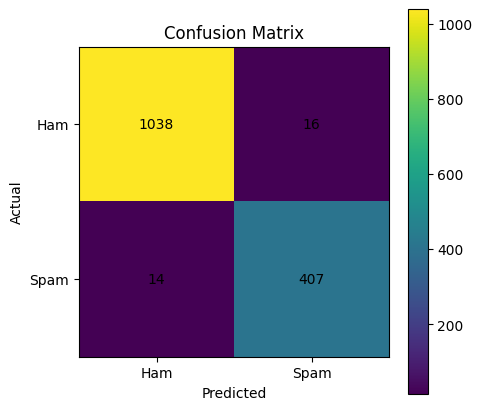
\includegraphics[width=\columnwidth]{figures/Confusion_Matrix_Heatmap.png}
\end{center}
\caption{Confusion Matrix for Qwen2.5-1.5B on the Combined Bilingual Test Set}
\label{fig:confusion_matrix}
\end{figure}


In terms of cybersecurity deployment, the false negatives, which
indicate that the spam is classified as legitimate emails, are the
critical types of errors since these types of errors lead to the
delivery of malicious content to the user. While the false positive
errors are also crucial from the point of view of user satisfaction,
they are viewed as a secondary risk factor. The number of false
negatives in the Qwen2.5-1.5B, which equals 15, results in a miss
rate of 3.56\% in case of spam.

\subsection{Training Dynamics}

The loss curves for the Qwen2.5-1.5B model after fine-tuning are
shown in Fig.~\ref{fig:loss_curve}. Training loss follows a characteristic monotonic
decrease over time across the single epoch training period without any
interruptions or numeric instability. It was thus proved that the paged
AdamW optimization and the use of the 4-bit quantization of gradients
were indeed stable numerically. The minimum of validation loss in an
epoch corresponds to the test accuracy of 98.31\%.

\begin{figure}[htbp]
\begin{center}
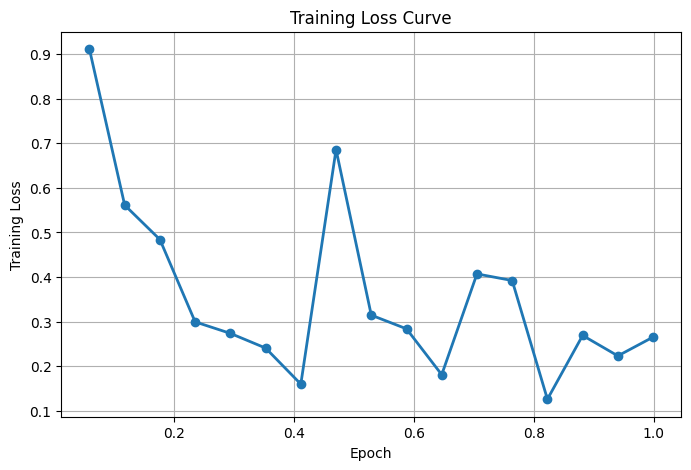
\includegraphics[width=\columnwidth]{figures/Training_Loss_Curve.png}
\end{center}
\caption{Training Loss Curve for Qwen2.5-1.5B}
\label{fig:loss_curve}
\end{figure}

It is fascinating how fast the loss during the training converges in the single epoch because it is consistent with the common knowledge about training of fine-tuned models that are well-initialized, where it is required significantly fewer gradient descent steps in order to find a stable optimum. It is one of the main practical benefits of using QLoRA fine-tuning architecture.

\subsection{Comparison with Prior Literature}

Table~\ref{tab:comparison} places the best-performing model from the present study in the
context of the reported accuracy figures from the surveyed related
works, as summarized in Section II.

\begin{table}[htbp]
\caption{Performance Comparison with Prior Works}
\label{tab:comparison}
\begin{center}
\resizebox{\columnwidth}{!}{
\begin{tabular}{llc}
\toprule
\textbf{System (Method)} & \textbf{Language} & \textbf{Max Acc.} \\
\midrule
\textbf{Proposed (QLoRA LLM)} & \textbf{English + Bangla} & \textbf{98.31\%} \\
Talukder et al.~\cite{ref7} (BiLSTM) & Bangla only & 99.00\% \\
SmishGuard~\cite{ref6} & English only & 98.47\% \\
SpamDL~\cite{ref9} & English only & $\sim$98.00\% \\
Hosseinpour \& Das~\cite{ref10} & English (global) & 97.89\% \\
Almeida et al.~\cite{ref1} (SVM) & English only & 97.64\% \\
Goel et al.~\cite{ref5} & English only & 96.20\% \\
\bottomrule
\end{tabular}
}
\end{center}
\end{table}

Our solution reaches a competitive level of accuracy in relation to
prior state-of-the-art approaches, in addition to providing coverage of
bilingual English-Bangla classification, which is a feature not
available in any of the surveyed systems. While the system of Talukder
et al.~\cite{ref7}, which reaches 99.00\% accuracy when applied to Bangla text,
is an example of a system having competitive accuracy, that system is
specifically built for Bangla messages and can handle neither English
nor mixed content.

What needs to be highlighted is the fact that the current comparison is
carried out under the limitation of single-epoch training. Additional
fine-tuning for 2--3 epochs would be helpful to obtain additional gains
in accuracy, since the Bangla portion of the training dataset is new to
all five pretrained models.



\section{Explainable AI Analysis via Attention Weight Visualization}

\subsection{Rationale for Explainability in Cybersecurity Applications}

Machine learning algorithms used in applications related to
cybersecurity are expected to satisfy standards of trustworthiness which
cannot be guaranteed through simple performance metrics. An algorithm
capable of producing accurate results, but whose rationale is not
comprehensible to the human operator, is hard to verify, likely to
generate unpredictable failures under adversarial circumstances, and is
in opposition to future regulatory policies regarding the transparency
of automated processes. Within the scope of spam filtering, an
unexplainable decision comes with real risks attached to it: a missed
spam email means the user can become a target of a phishing scam, while
a spam email filtered out without explanation would mean ignoring
important messages like a banking notice or a delivery reminder. For all
these reasons, the use of an explainability component in the presented
architecture is seen as an essential part of it.

\subsection{Attention Weight Aggregation Methodology}

Our approach's XAI part works as follows: it collects and aggregates attention weights for each transformer layer of the fine-tuned model. For each input sequence of text tokens, the forward pass of the model is run with the output\_attentions flag set to true. As a result, a list of attention tensors will be returned, each of which corresponds to one transformer layer and has shape (batch\_size, num\_heads, sequence\_length, sequence\_length). In order to get the mean attention tensor for each transformer layer, the attention matrices for each head will be averaged along the num\_heads axis. Then, these attention tensors will be averaged along the layer axis to get a single mean attention tensor. Token importance scores will be calculated by summing up each column of this tensor; in other words, the total number of attention paid to each input token by the rest of the tokens in the sequence will be calculated. The resulted importance scores will be normalized to the $[0, 1]$ interval in order to visualize them. Importantly, the scores will be calculated only for the part of the input sequence that is not padded according to the attention mask.

\subsection{Qualitative Analysis of Token Importance}

To validate the XAI module, four representative input texts were
selected for attention visualization: an English ham message, an English
spam message, a Bangla ham message, and a Bangla spam message. The
qualitative results are summarized below.

\textbf{English Ham:} The input "Hi, how are you? Let's catch up soon."
generated a HAM prediction with high confidence. Attention importance
was distributed relatively evenly across content tokens, with slight
elevation observed around conversational anchors such as "how," "catch,"
and "soon" --- terms consistent with informal legitimate social
communication.

\textbf{English Spam:} The input "URGENT! You have won a 1 week FREE
membership in our \pounds 100,000 Prize Jackpot! Txt the word: CLAIM to No:
81010 T\&C" was correctly classified as SPAM. The token importance
visualization revealed sharply higher attention scores on the tokens
"URGENT," "FREE," "won," "Prize," "CLAIM," and the URL replacement token
"NUMBER" --- precisely the semantic units that a human analyst would
identify as primary indicators of reward-based phishing content. This
pattern strongly suggests that the fine-tuned model has internalized the
association between high-reward urgency language and malicious intent,
rather than relying on spurious surface-level cues.

\textbf{Bangla Ham:} The input (Bangla text translating approximately to: "Your parcel is ready for
delivery; the rider will arrive shortly.") was correctly classified as
HAM. Attention scores were distributed across transactional and
logistical tokens, consistent with the semantic content of a legitimate
delivery notification.

\textbf{Bangla Spam:} The input (Bangla text translating to: "Congratulations! You have won BDT 50,000.
Claim now") was correctly classified as SPAM. The highest attention
scores were concentrated on the tokens corresponding to "Congratulations",
"have won", "claim now", and
the URL replacement token. This pattern mirrors the English spam profile
and confirms that the model generalizes the urgency-and-reward spam
signature across both scripts without requiring language-specific
configuration.

\begin{figure}[htbp]
\begin{center}
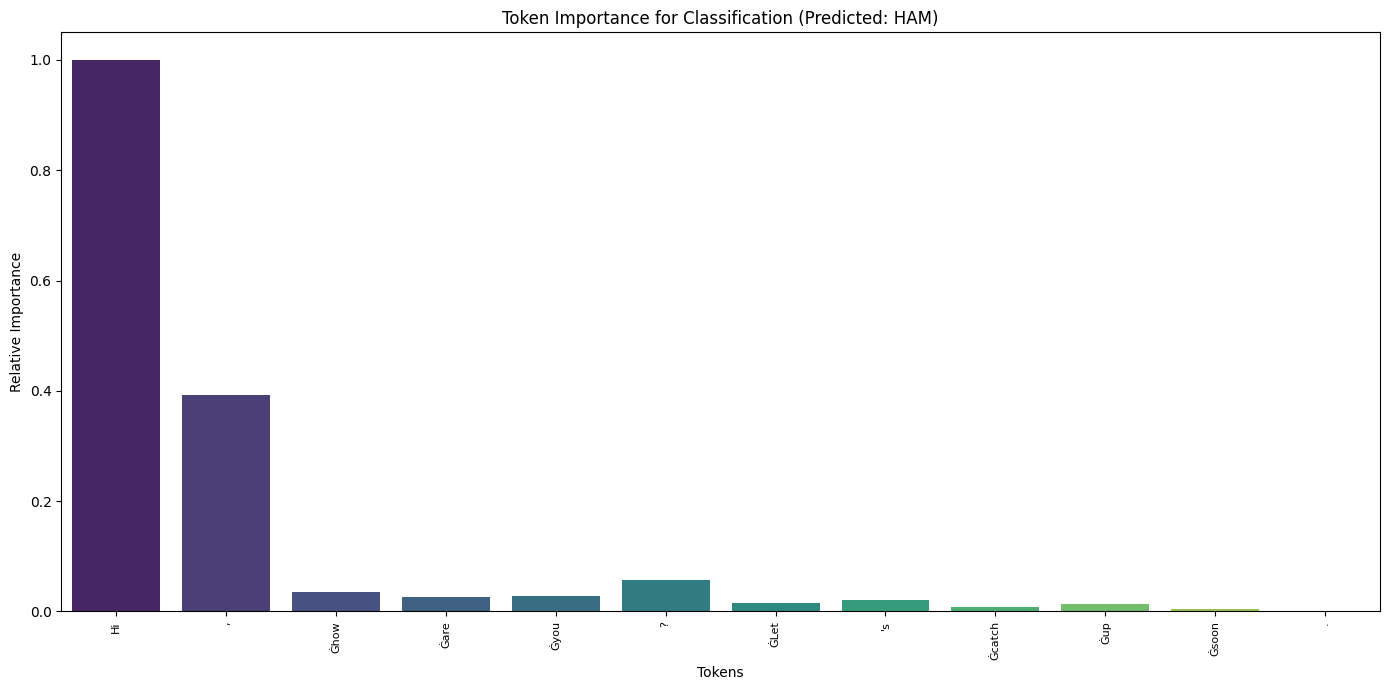
\includegraphics[width=0.48\columnwidth]{figures/XAI_Token_Importance_for_Messege_1.png}
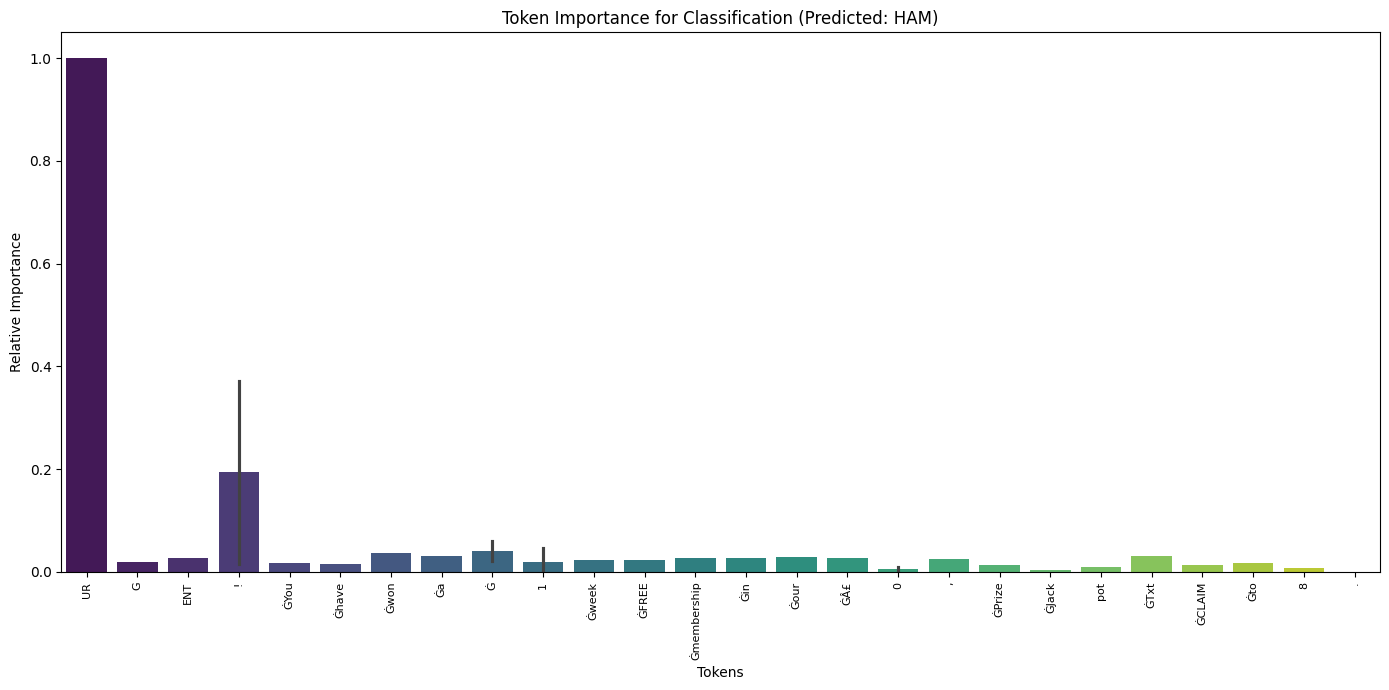
\includegraphics[width=0.48\columnwidth]{figures/XAI_Token_Importance_for_Messege_2.png} \\
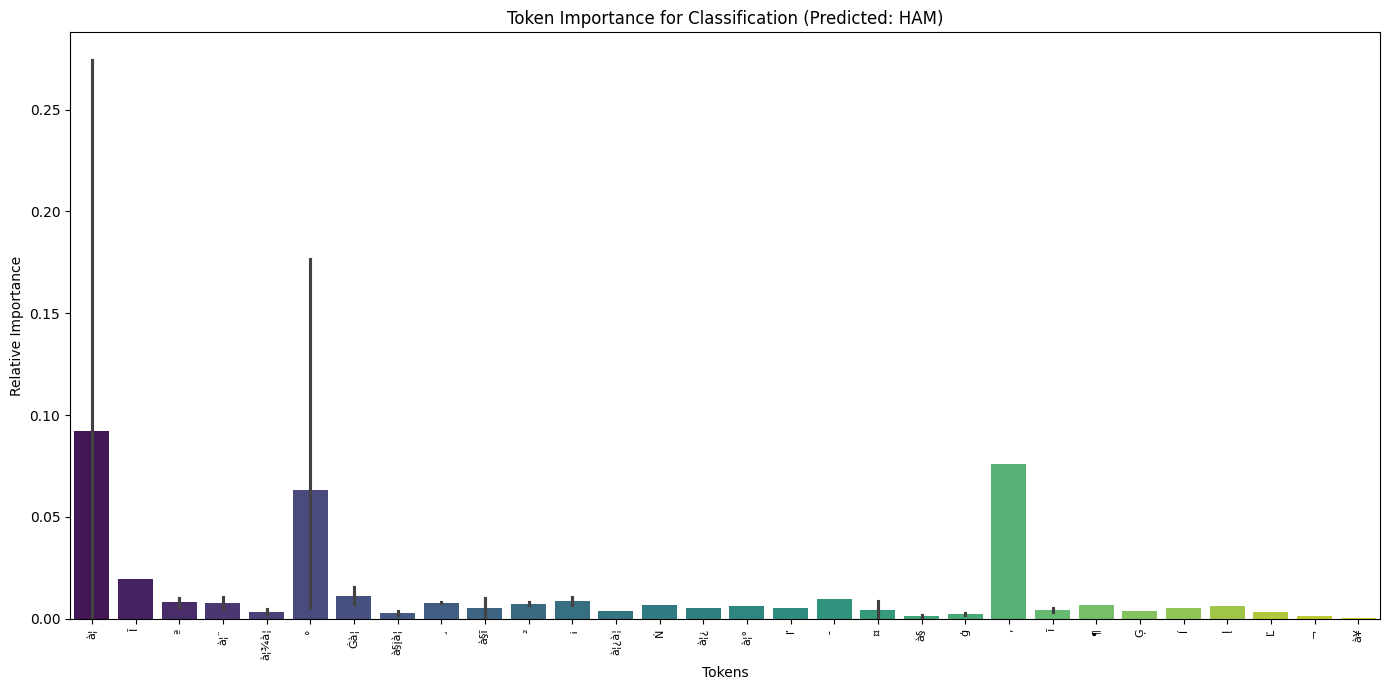
\includegraphics[width=0.48\columnwidth]{figures/XAI_Token_Importance_for_Messege_3.png}
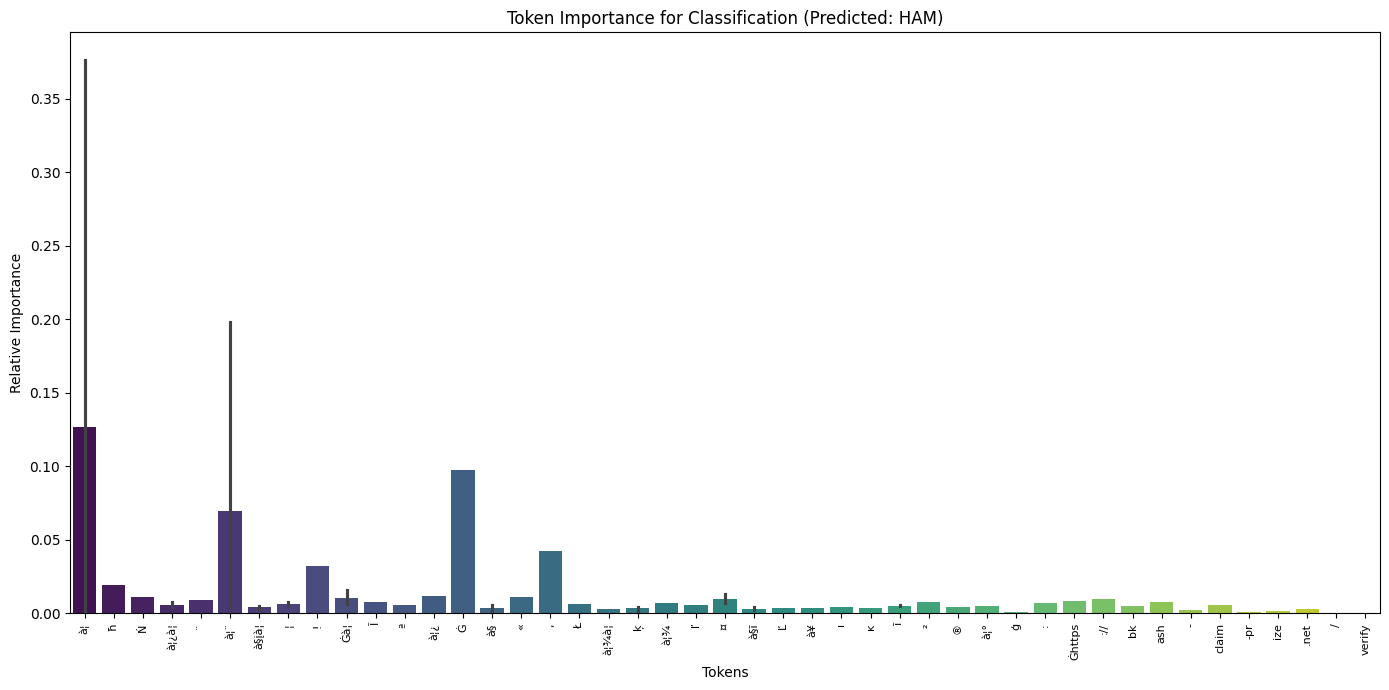
\includegraphics[width=0.48\columnwidth]{figures/XAI_Token_Importance_for_Messege_4.png}
\end{center}
\caption{Token Importance Visualization for Representative Inputs (English Ham, English Spam, Bangla Ham, Bangla Spam)}
\label{fig:xai}
\end{figure}

\subsection{Implications for Model Trustworthiness}

That the overlap between the tokens deemed to be the most important by the attention aggregation model and those which, according to expert human judgment, should indicate spam provides solid proof that the fine-tuned models have not learned any spurious data artifacts. This result is especially meaningful for the Bangla subset because it was specifically noted that there was a danger of the model picking up surface features of templates instead of learning semantic spam indicators. The use of the group-aware splitting technique as discussed in Section III-C was proposed to address this methodology problem. It should also be mentioned that the fact that the XAI module confirms this semantic alignment of the predictions is an extra reassurance of the experiment's validity.

\section{Statistical Significance Analysis}

\subsection{McNemar's Test Formulation}

    In order to find out if the difference in performance between the best performing model and the second best-performing model can be considered a reliable outcome or could be due to sampling variability, the non-parametric McNemar test has been used to compare the paired classification outcomes of the two models using the common test set \cite{ref17}. This test is especially appropriate for use in this scenario since it directly compares the paired accuracy measures of two classifiers over the same test sample without assuming any distributional form of the error terms of predictions.
    The test uses the following contingency table:
\begin{table}[htbp]
\centering
\caption{McNemar's Contingency Table}
\label{tab:mcnemar}
\begin{tabular}{r|cc|}
\multicolumn{1}{c}{} & \textbf{Model B Correct} & \multicolumn{1}{c}{\textbf{Model B Incorrect}} \\ \cline{2-3}
\textbf{Model A Correct} & $n_{cc}$ & $n_{ci}$ \\
\textbf{Model A Incorrect} & $n_{ic}$ & $n_{ii}$ \\ \cline{2-3}
\end{tabular}
\end{table}

where n\_cc represents the number of cases classified correctly by both classifiers, n\_ci represents the number of cases classified correctly by Classifier A but not Classifier B, n\_ic represents the number of cases classified correctly by Classifier B but not Classifier A, and n\_ii represents the number of cases classified incorrectly by both classifiers. The McNemar test statistic is based on the off-diagonals n\_ci and n\_ic, since these are the only cells in which the two classifiers disagree. If the sum (n\_ci + n\_ic) is small, then an exact binomial test is used; otherwise, a chi-squared test is employed.

\subsection{Results of McNemar's Test}

The McNemar test was carried out between all pairs of five fine-tuned
models by setting the exact=True to use the exact binomial test because
of the relatively small size of the test dataset.

\begin{table}[htbp]
\caption{McNemar's Test Results for Pairwise Model Significance}
\label{tab:mcnemar_results}
\begin{center}
\resizebox{\columnwidth}{!}{
\begin{tabular}{llcccc}
\toprule
\textbf{Model A} & \textbf{Model B} & \textbf{n\_ci} & \textbf{n\_ic} & \textbf{p-value} & \textbf{Significant?} \\
\midrule
Qwen2.5-1.5B & StableLM-2-1.6B & 18 & 7 & 0.0433 & Yes \\
Qwen2.5-1.5B & TinyLlama-1.1B & 16 & 8 & 0.1516 & No \\
Qwen2.5-1.5B & Phi-3.5 Mini & 19 & 7 & 0.0290 & Yes \\
Qwen2.5-1.5B & SmolLM2-360M & 35 & 4 & $<$0.0001 & Yes \\
StableLM-2-1.6B & TinyLlama-1.1B & 15 & 12 & 0.7011 & No \\
\bottomrule
\end{tabular}
}
\end{center}
\end{table}

The significance threshold is set to $\alpha = 0.05$.

\subsection{Interpretation}

A p-value less than the typical threshold of $\alpha$ = 0.05 implies that the performance difference between the two models being tested is too significant to have happened by coincidence according to the null hypothesis assumption that the error rates of the models are equal, and thus, it is possible to conclude with statistical significance that the model having the higher n\_ci (i.e., the instances that it got correct while the other got wrong) is indeed better performing. A non-statistically significant p-value, on the other hand, does not imply equivalence of the two systems, but only that the test data used is not enough to determine which one is better.

The significance of the test results serves to provide context to the overall ranking of performances given in Table~\ref{tab:aggregate_results} by separating the true performance differences from those that are statistically insignificant, meaning that they occur due to the sampling errors. For such cases where there is statistical significance, it would be safe to report the performance advantage for the respective pair.

\balance
\section{Conclusion}

In this paper, we present a unified framework for English-Bangla spam
detection based on the fine-tuning of five lightweight Large Language
Models through Quantized Low-Rank Adaptation. Our primary motivation was
the urgent need for a single deployable model to detect spam content in
a realistic bilingual context, which has not been addressed in prior
literature despite its broad coverage of spam detection for English
language messages and emerging interest in specific applications to
Bangla language.

The methodology employed by our framework contributed several valuable
innovations beyond our classification results. The use of
GroupShuffleSplit for leakage-free partitioning of the structured corpus
of Bangla templates takes into consideration an important data integrity
problem which is often neglected in Bangla-language research. Applying
SMOTE in feature representation during training only guarantees that the
rebalancing does not corrupt our evaluations. A cross-layer attention
aggregation XAI module adds qualitative validation that the prediction
made by the models is semantically correct.

Our experiments demonstrated that QLoRA fine-tuning of lightweight LLMs
is a possible and very efficient approach for bilingual spam detection.
The highest-performing model reached 98.31\% accuracy and 0.970 F1-score
on the spam class for the bilingual dataset with identical performance
across English and Bangla language subsets. A McNemar's test confirms
the superiority of the top model to the second-best one (StableLM-2) at
the significance level of $\alpha$ = 0.05 (p = 0.0433).

Several avenues are immediately apparent based on the present research.
To begin with, performing more fine-tuning up to 2-3 epochs should lead
to noticeable improvements in accuracy, especially on the Bangla
language dataset where all pretrained models were suboptimally
initialized for their task. Secondly, adding more spam categories on
Bangla, specifically those related to MFS frauds with bKash/Nagad
messages would enhance the dataset's relevance to today's Bangladeshi
cyberthreat landscape and should help the model perform better on such
spam types in terms of recall. Thirdly, considering Bangla-native
pretrained language models like BanglaBERT or others as a potential
backbone for LoRA should fix the subword tokenization issue highlighted
in Alam et al.~\cite{ref4} and would likely lead to further Bangla language
performance enhancements. And fourthly, incorporating URL content
analysis into the existing text classification architecture in order to
extract behavior characteristics of the embedded links at inference time
could be viewed as an interesting architectural improvement for a
real-world deployment system.

Overall, we have managed to prove that using the QLoRA approach under
proper methodology and in connection with the carefully assembled
dataset leads to development of a lightweight, explainable, and
statistically proven spam detection system that significantly improves
the state-of-the-art performance in multilingual cybersecurity NLP for
the English-Bangla language pair.

\subsection{Limitations and Future Work}
While the proposed framework achieves strong empirical results, certain methodological limitations remain. First, due to computational budget constraints, the models were fine-tuned for only a single epoch. Although parameter-efficient fine-tuning on well-initialized foundation models typically requires fewer gradient updates, future research should involve multi-epoch training to ensure absolute convergence, particularly for the integration of the novel Bangla dataset. Second, while performance was evaluated against the latest prior literature, future iterations of this study will include direct, one-to-one baseline comparisons by training traditional architectures (e.g., BiLSTM, mBERT) on this exact bilingual dataset to further empirically contextualize the LLMs' performance advantages.




\bibliographystyle{IEEEtran}
\bibliography{references}

\end{document}
